\chapter{Testes e resultados}

Neste capítulo estão relacionados os testes realizados para validar o funcionamento e a eficácia do aplicativo ColetaCacau, bem como os resultados obtidos após a implementação das funcionalidades de coleta de dados com RFID. A análise dos resultados foca na eficiência da coleta de dados em campo, redução de erros humanos, e na integração das funcionalidades com a plataforma web e a API.

\section{Testes Realizados}

Os testes foram realizados em três principais componentes do sistema: o aplicativo móvel (ColetaCacau), a plataforma web (PlataformaCacau) e a API. Abaixo estão descritos os principais cenários de teste e seus resultados:

\subsection{Testes no Aplicativo Móvel}

\subsubsection{Identificação Automática de Árvores com RFID}
Testou-se a leitura de tags RFID para garantir que o aplicativo reconhecesse automaticamente cada árvore. O teste validou a capacidade do aplicativo de vincular as árvores aos dados corretos da coleta, eliminando a necessidade de identificação manual.

A Figura \ref{fig:RfidTest01} ilustra como as tags RFID foram anexadas às árvores. Cada tag inicial contém informações visuais adicionais, como o nome da fazenda, área homogênea, unidade operacional e ponto amostral associados. Esses detalhes garantem que cada tag seja corretamente vinculada à árvore correspondente, promovendo precisão no processo de identificação e coleta. Foram testadas 140 tags, todas já anexadas às suas respectivas árvores. 

Para se ter ideia de custos, para cada área homogênea de cacau em uma propriedade são necessárias 35 plantas participantes da coleta. Esse valor pode aumentar um pouco a depender dos resultados observados. Uma área homogênea é aquela em que a produção de amêndoas é  próxima para todas as árvores, levando em consideração também outras variáveis como solo e tipo de cacau plantado. Geralmente, em 1 hectare são plantados aproximadamente 1000 plantas de cacau. 

\begin{figure}[H]
    \centering
    %\frame{
    \frame{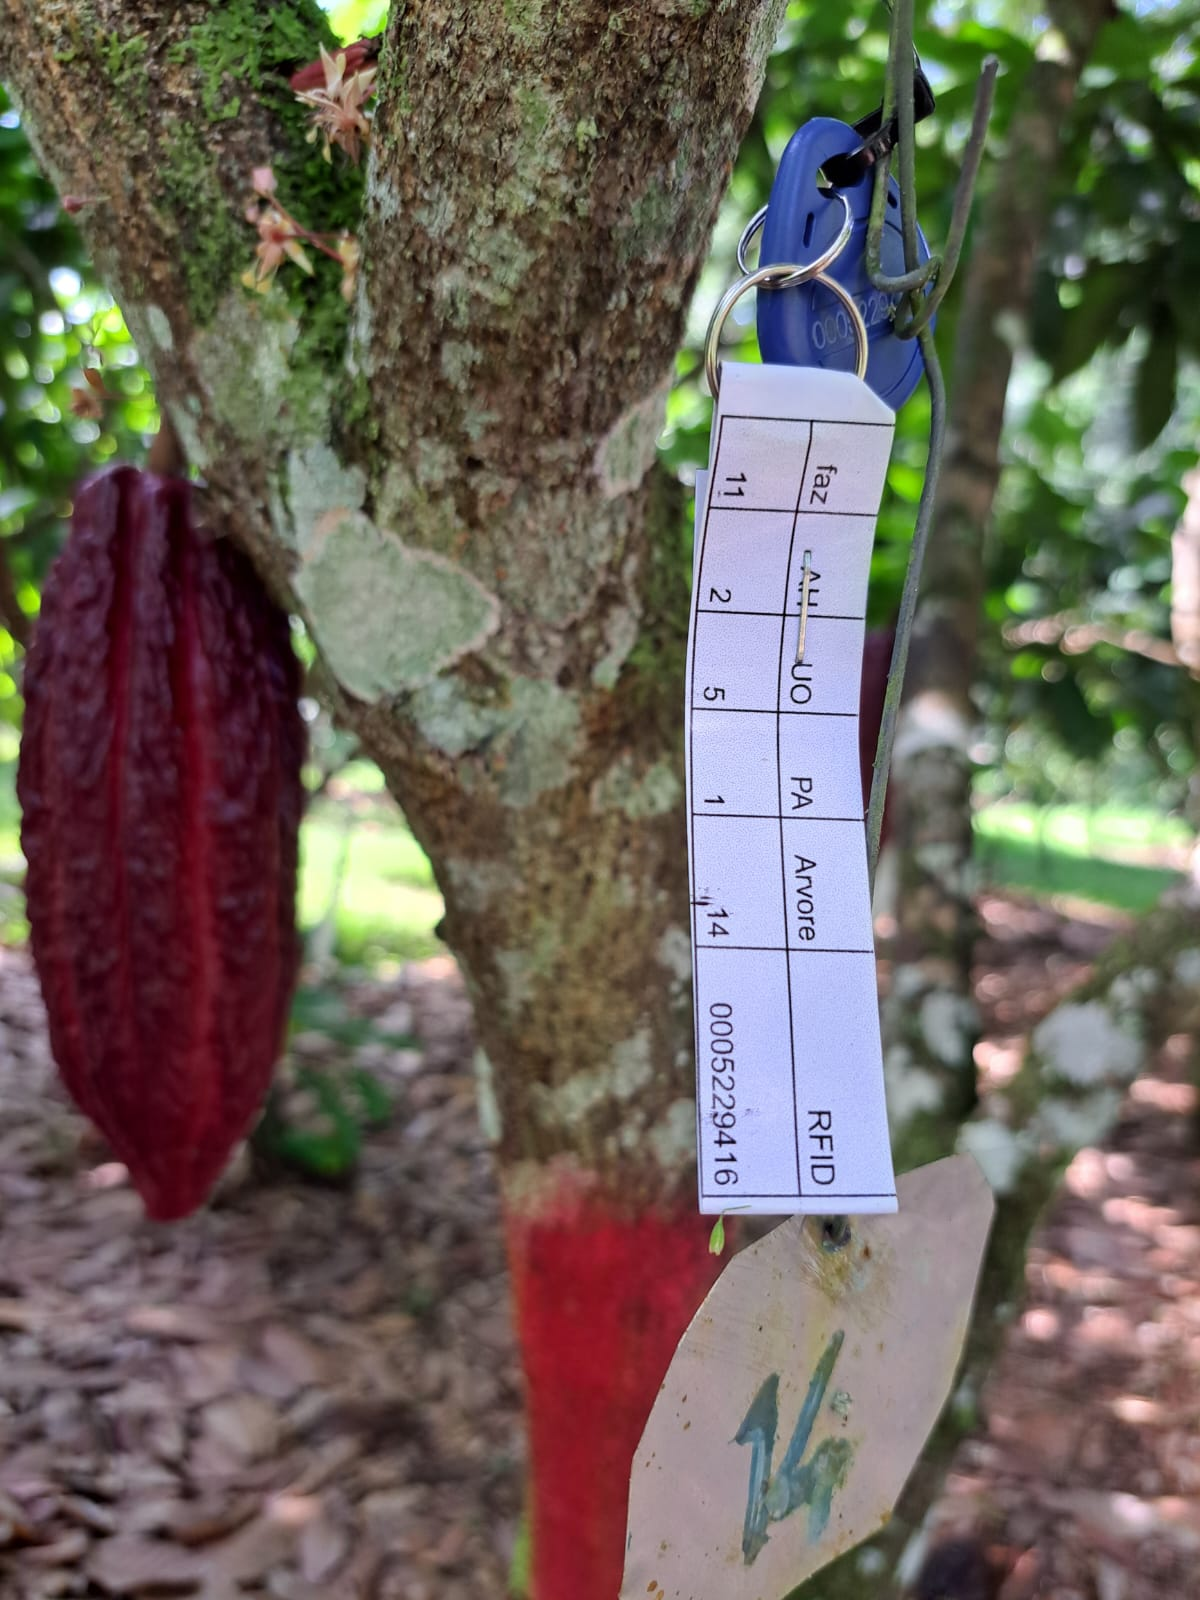
\includegraphics[width=0.4\textwidth]{images/rfid/rfid-test-01.jpeg}}\\
     \caption{Tag RFID vinculada a uma árvore, com informações adicionais para identificação.}
     Autora: Marta M. Dornelles, 2024.
    \label{fig:RfidTest01}
\end{figure}

Já a Figura \ref{fig:RfidTest02} demonstra o momento em que o aplicativo realiza a leitura da tag e consulta a base de dados \textit{offline}. Nesse processo, o sistema encaminha automaticamente o coletor para a tela correspondente à árvore lida, agilizando a navegação e garantindo a consistência na coleta de dados.

\begin{figure}[htb]
    \centering
    \frame{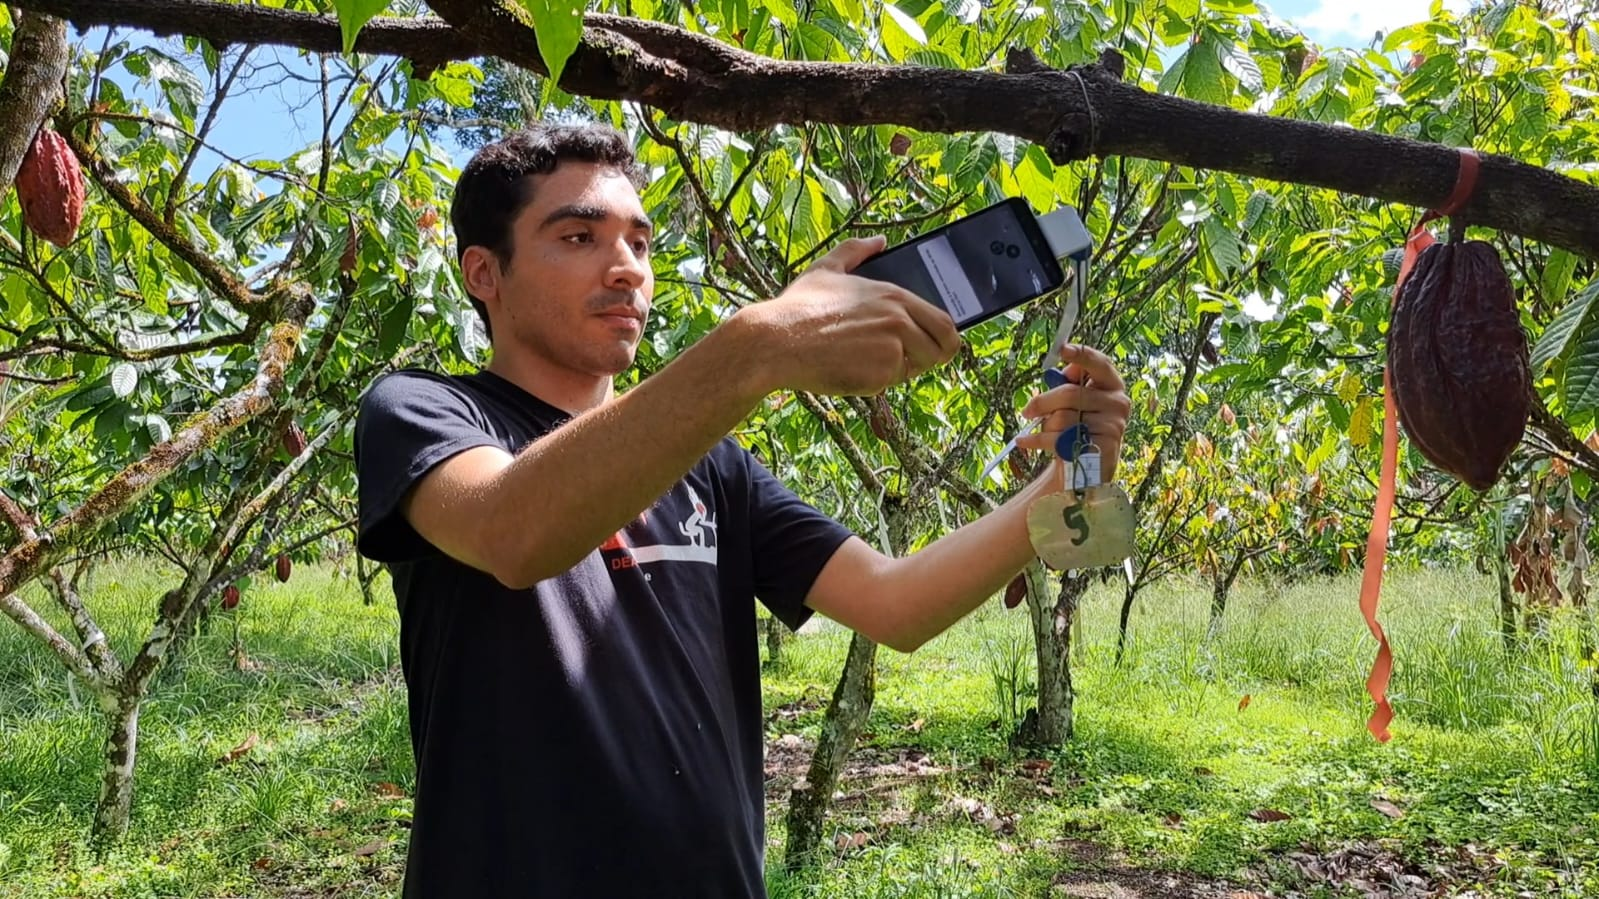
\includegraphics[width=0.7\textwidth]{images/rfid/rfid-test-02.jpeg}}
        \caption{Tela de consulta à tag RFID e direcionamento para os dados correspondentes da árvore.}
     Autora: Marta M. Dornelles, 2024.
    \label{fig:RfidTest02}
\end{figure}

\subsubsection{Coleta \textit{Offline} e Sincronização de Dados}
Avaliou-se a capacidade do aplicativo de coletar dados \textit{offline} e sincronizá-los com o servidor quando uma conexão fosse restabelecida. O teste confirmou que os dados coletados em campo são armazenados no banco de dados local (\textit{RealmDB}) e sincronizados corretamente.

\subsubsection{Validação de Dados da Coleta}
Realizou-se uma série de testes para validar a entrada de dados, assegurando que o aplicativo impedisse o envio de dados incompletos ou inconsistentes. O teste verificou o preenchimento correto de todos os campos obrigatórios antes de salvar ou sincronizar os dados.

\subsection{Testes na Plataforma Web}
\subsubsection{Cadastro e Atualização de RFIDs}
Testou-se o fluxo de cadastro e atualização de códigos RFID através da interface web, garantindo que o gestor pudesse criar e modificar os códigos das tags com facilidade e precisão. Foram feitas validações para não permitir inclusão de códigos de tags que já existissem em uma determinada propriedade vinculada àquele usuário.

\subsubsection{Vinculação de RFIDs com Árvores}
Validou-se o processo de vinculação dos RFIDs cadastrados às árvores específicas, tanto no cadastro inicial quanto na atualização de informações. Os testes garantiram que o código RFID correto fosse associado à árvore correspondente, permitindo a identificação precisa no campo.

\subsubsection{Listagem e Edição de Árvores}
A funcionalidade de listagem e edição de árvores foi testada para garantir que as informações fossem exibidas de maneira clara, permitindo ao gestor atualizar os dados conforme necessário.

\subsection{Testes na API e Banco de Dados}
\subsubsection{Criação e Atualização de RFIDs}
Testou-se os \textit{endpoints} de criação, atualização, listagem, visualização, associação e desassociação de RFIDs com árvores, garantindo que o sistema mantivesse a integridade dos dados e refletisse as alterações na plataforma web e no aplicativo.

\subsubsection{Exportação dos Dados da Coleta}
Avaliou-se a exportação dos dados coletados, incluindo o campo RFID vinculado às árvores. O teste confirmou que os dados exportados incluíam as informações corretas, facilitando a análise pelos gestores.

\section{Resultados Obtidos}
A implementação da tecnologia RFID no processo de coleta de dados representou um marco importante na eficiência e na precisão das operações em campo. Antes da adoção dessa tecnologia, os coletores enfrentavam desafios significativos na localização das árvores, o que envolvia um padrão de deslocamento confuso e ineficaz, frequentemente descrito como um trajeto em “zig-zag”. Esse método, além de consumir mais tempo e energia, contribuía para o aumento de erros na identificação das árvores e na coleta de informações, comprometendo a confiabilidade dos dados.

Com a introdução das tags RFID, cada árvore passou a ser identificada de forma única e automática, eliminando a necessidade de movimentações desordenadas. Agora, os coletores conseguem localizar rapidamente as árvores marcadas, utilizando leitores RFID que fornecem informações precisas e em tempo real. Essa mudança resultou em uma significativa economia de tempo, permitindo que o foco dos coletores fosse direcionado à coleta de dados propriamente dita, sem distrações ou esforços desnecessários.

Os benefícios dessa abordagem vão além da economia de tempo. A automatização do processo trouxe uma redução considerável dos erros humanos, anteriormente comuns devido à identificação manual ou a métodos visuais imprecisos. Com o RFID, a identificação das árvores tornou-se padronizada e consistente, promovendo maior confiabilidade e uniformidade nos dados coletados. Essa melhoria não apenas elevou a qualidade do trabalho realizado, mas também contribuiu para análises mais precisas e decisões informadas em etapas subsequentes do projeto.

Outro impacto relevante foi o aumento da produtividade dos coletores. Antes da implementação do RFID, o desgaste físico e mental causado pela movimentação desordenada e pela dificuldade em localizar as árvores comprometia o desempenho da equipe. Agora, com a otimização dos trajetos e a simplificação do processo, os coletores podem realizar suas tarefas com mais agilidade e menos esforço, gerando um ambiente de trabalho mais eficiente e satisfatório.

Além disso, a utilização do RFID trouxe ganhos indiretos, como a redução do custo operacional, uma vez que o tempo economizado por coleta possibilita a execução de mais tarefas em menos tempo. A confiabilidade nos dados também facilita a integração com sistemas de análise automatizada, como ferramentas de \textit{big data} ou inteligência artificial, abrindo caminho para futuras inovações no gerenciamento de informações.

\section{Seções de Imagens}
Para ilustrar o funcionamento do ColetaCacau e as funcionalidades implementadas na plataforma web e no aplicativo móvel, a seguir são apresentadas capturas de tela detalhando as principais interfaces e fluxos do sistema.

\subsection{Imagens da Plataforma Web}

\subsubsection{Tela de Listagem de RFIDs}
A Figura \ref{fig:ListRfid} exibe todos os RFIDs cadastrados no sistema, permitindo que o gestor visualize rapidamente os códigos e os associe às árvores de maneira eficiente.

\begin{figure}[H]
    \centering
    \frame{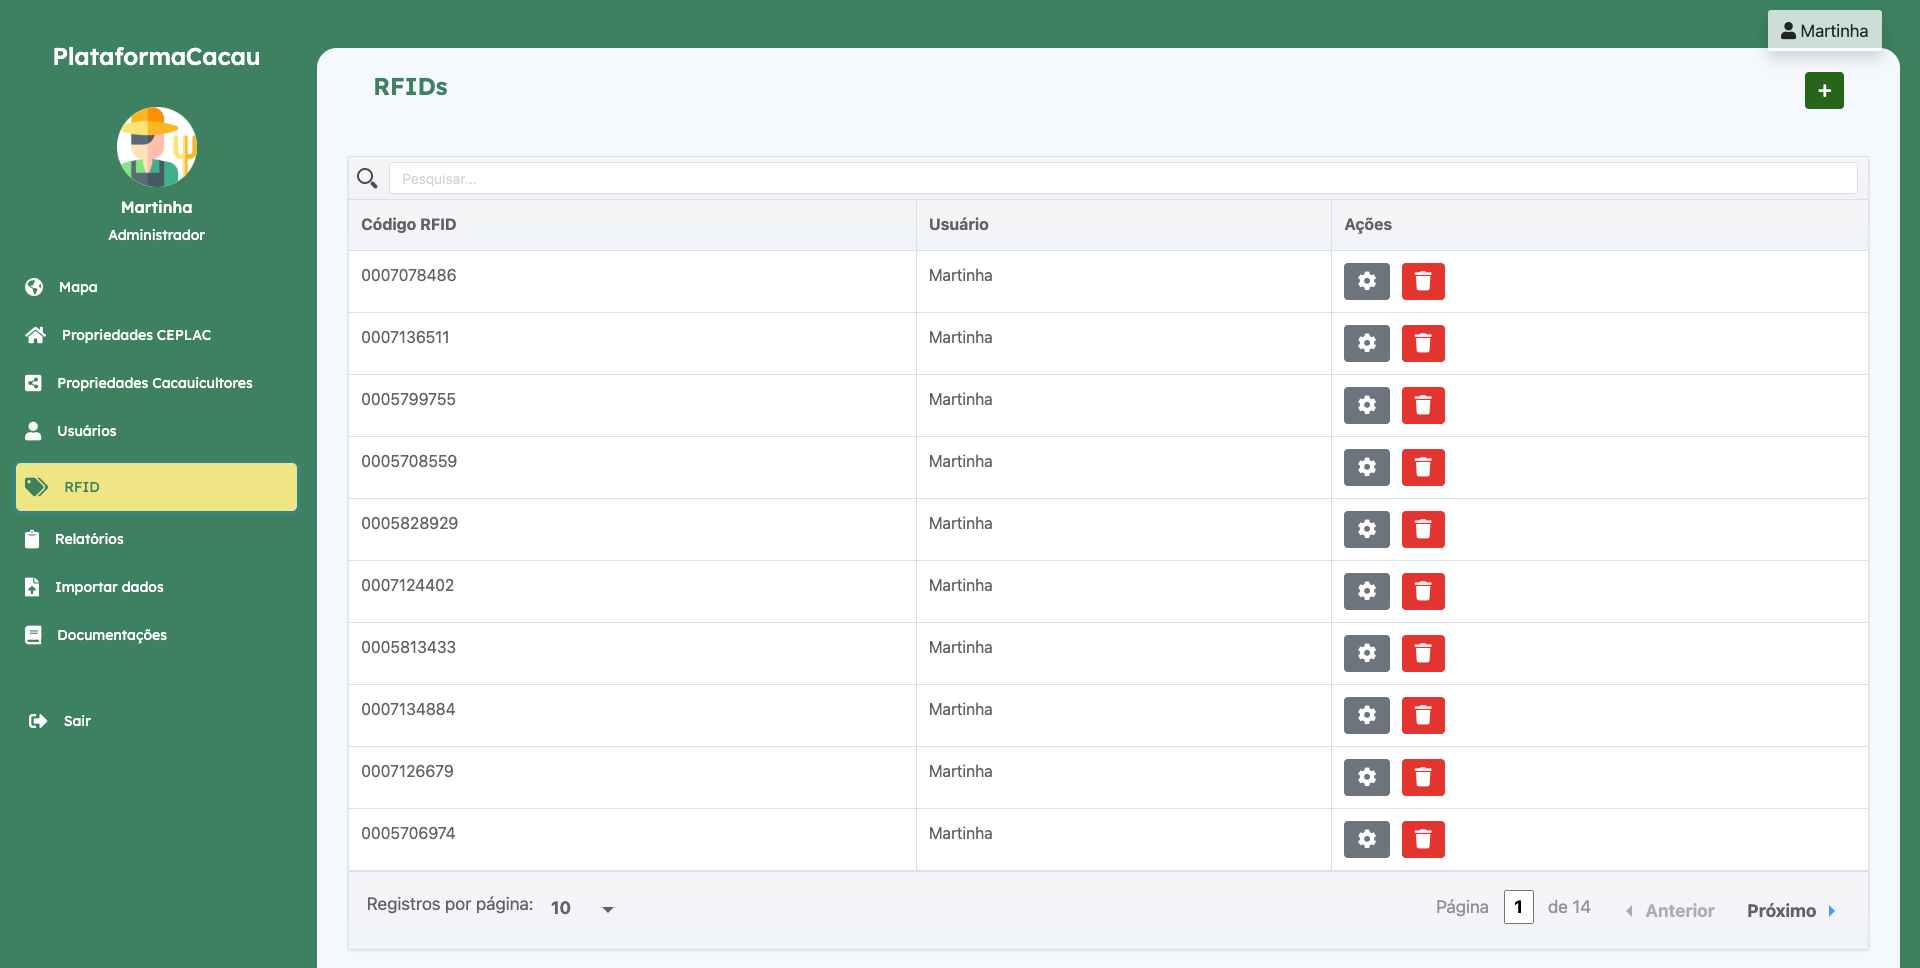
\includegraphics[width=\textwidth]{images/web/list-rfid.png}}
    \caption{Tela de listagem de RFIDs na plataforma web.}
    \label{fig:ListRfid}
\end{figure}

\subsubsection{Janela de Criação de Código RFID}
A Figura \ref{fig:CreateRfid} mostra a interface de cadastro de novos RFIDs, onde o gestor insere o código e outras informações necessárias para adicionar uma nova tag ao sistema.

\begin{figure}[H]
 \centering
 \frame{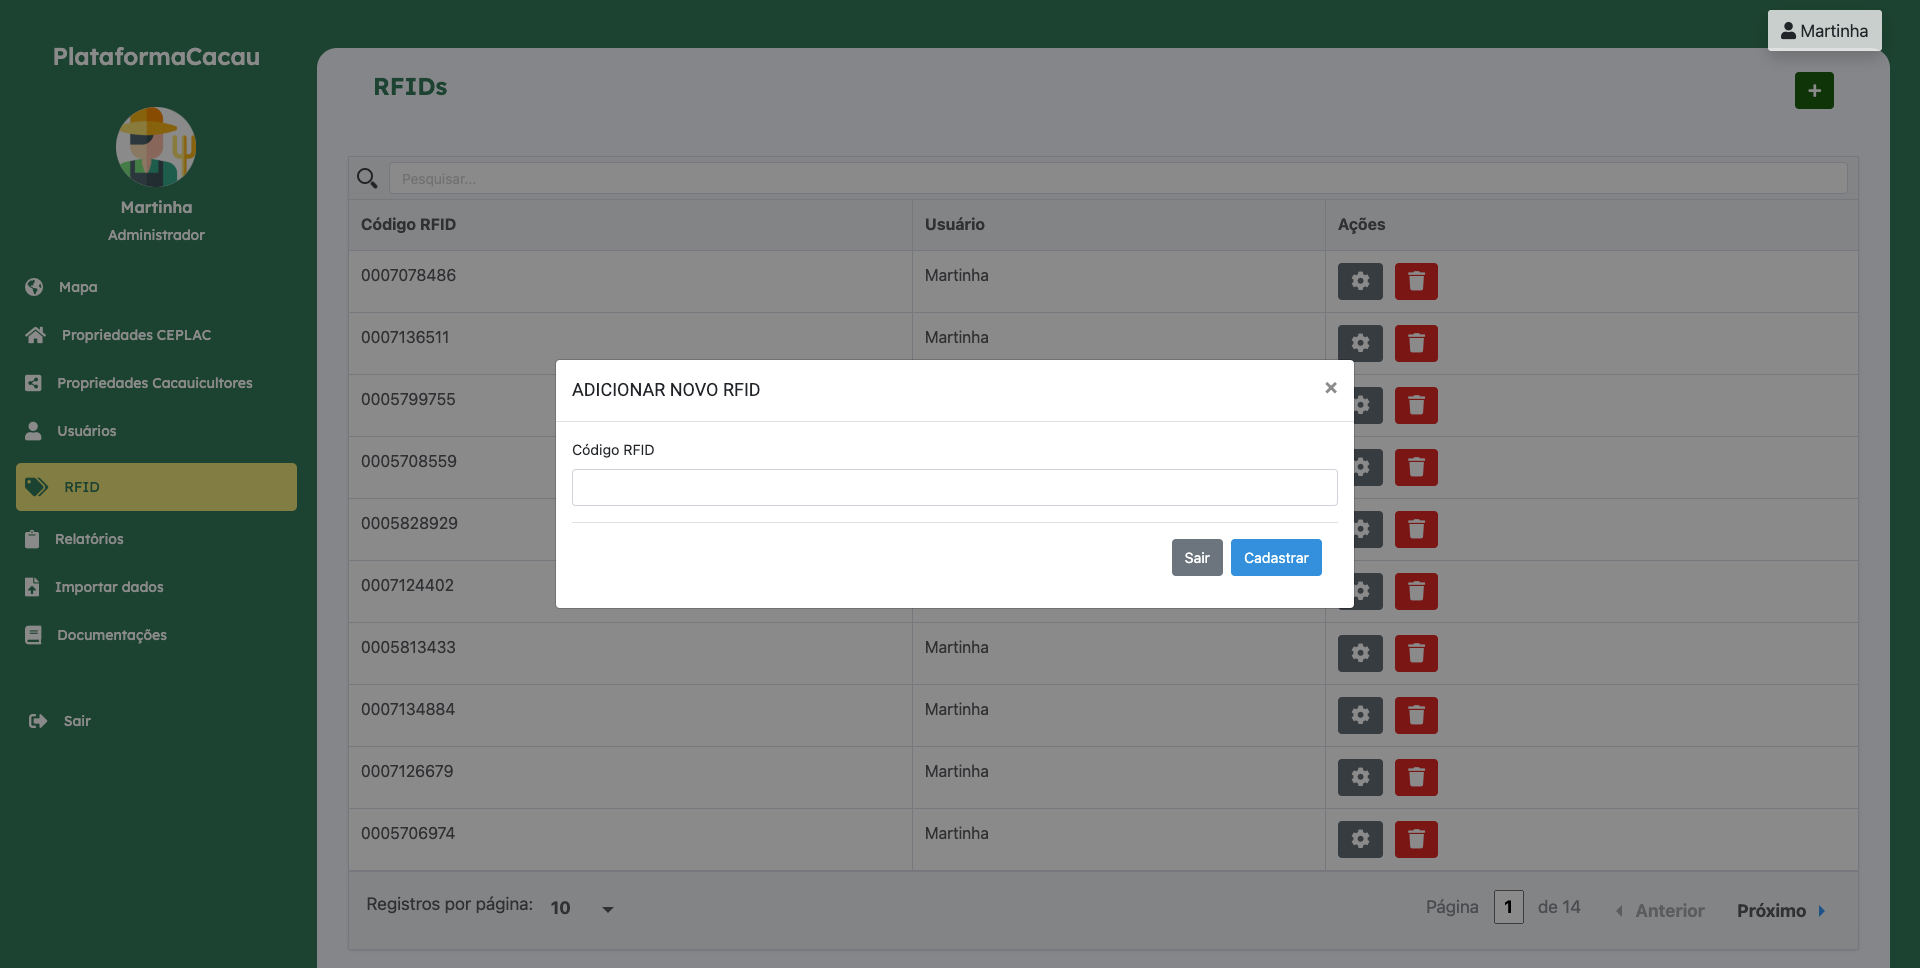
\includegraphics[width=\textwidth]{images/web/create-rfid.png}}
 \caption{Janela de criação de código RFID na plataforma web.}
 \label{fig:CreateRfid}
\end{figure}

\subsubsection{Janela de Atualização de Código RFID}
A Figura \ref{fig:UpdateRfid} representa a tela que permite ao gestor modificar as informações de um RFID existente, garantindo que o sistema reflita sempre as informações corretas.

\begin{figure}[H]
 \centering
 \frame{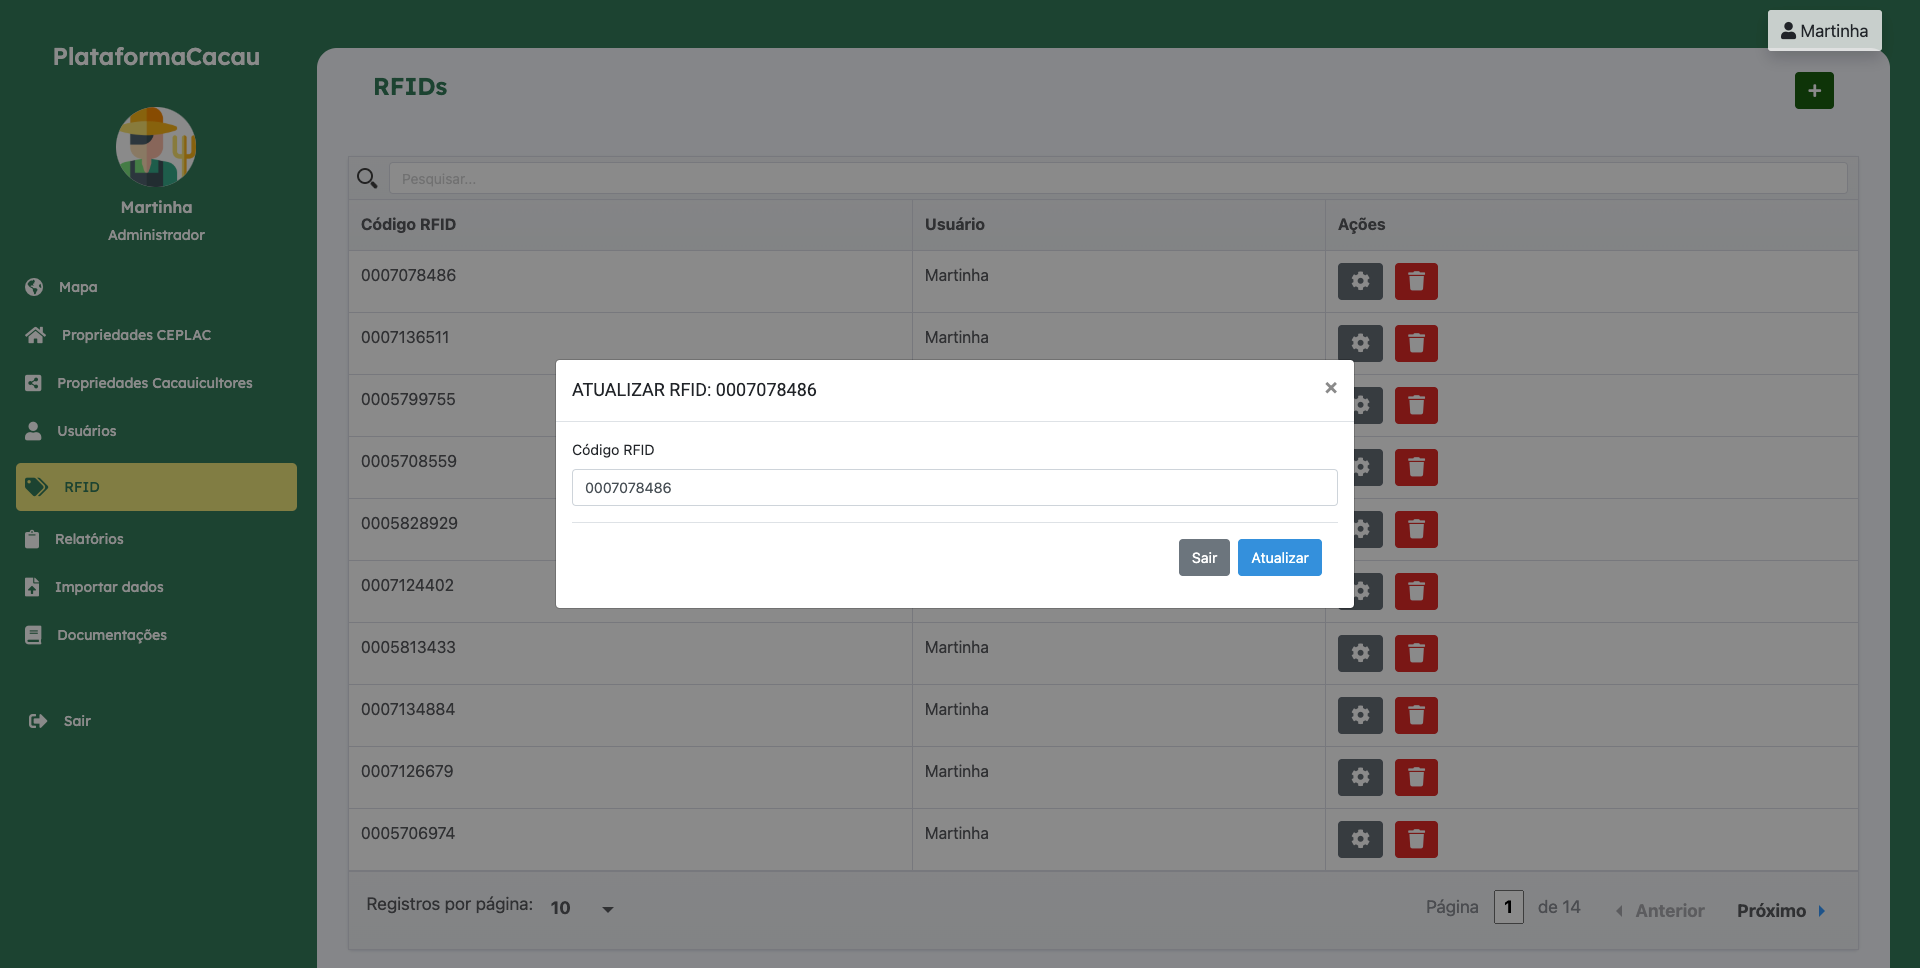
\includegraphics[width=\textwidth]{images/web/update-rfid.png}}
 \caption{Janela de atualização de código RFID na plataforma web.}
 \label{fig:UpdateRfid}
\end{figure}

\subsubsection{Tela de Listagem de Árvores}
A Figura \ref{fig:TreeList} exibe a lista completa de árvores cadastradas, com seus respectivos RFIDs, oferecendo uma visão geral organizada para o gestor.

\begin{figure}[H]
 \centering
 \frame{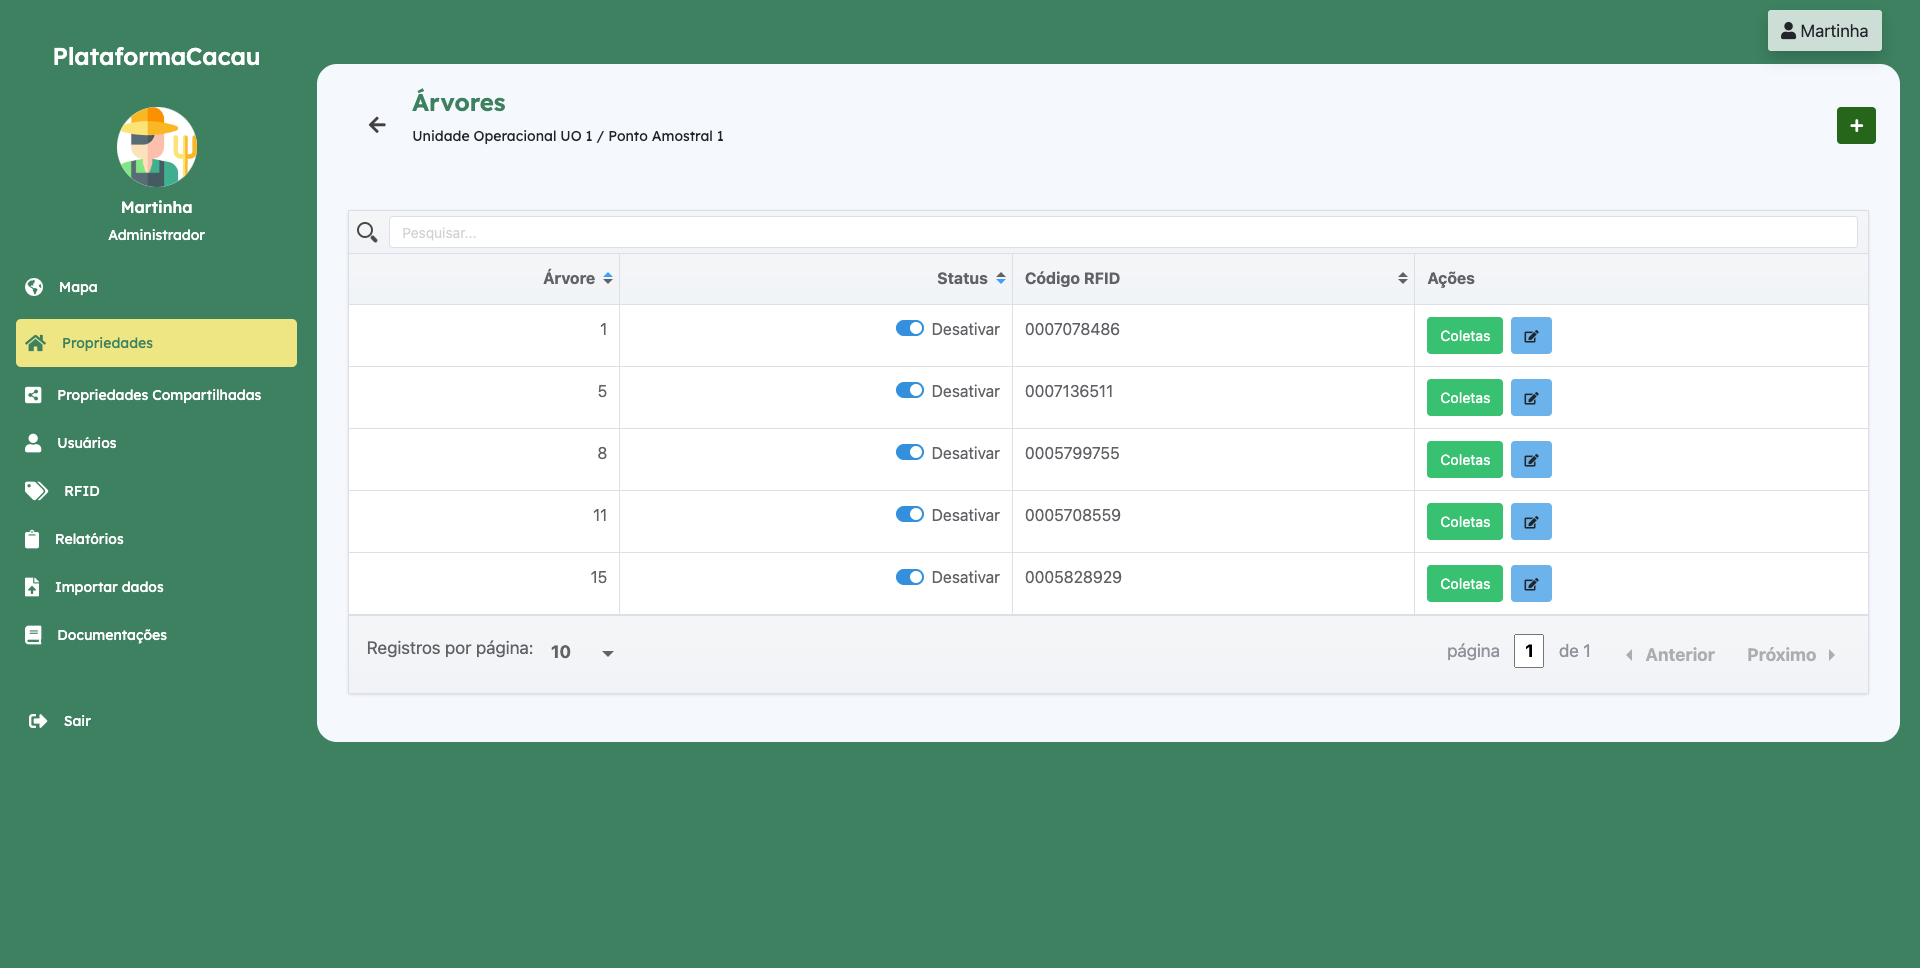
\includegraphics[width=\textwidth]{images/web/list-tree.png}}
 \caption{Tela de listagem de árvores na plataforma web.}
 \label{fig:TreeList}
\end{figure}

\subsubsection{Janela de atualização do código RFID da árvore}
A Figura \ref{fig:UpdateTreeRfid} representa a interface onde o gestor pode atualizar o código RFID vinculado a uma árvore específica, facilitando o gerenciamento e manutenção das tags associadas.

\begin{figure}[htb]
 \centering
 \frame{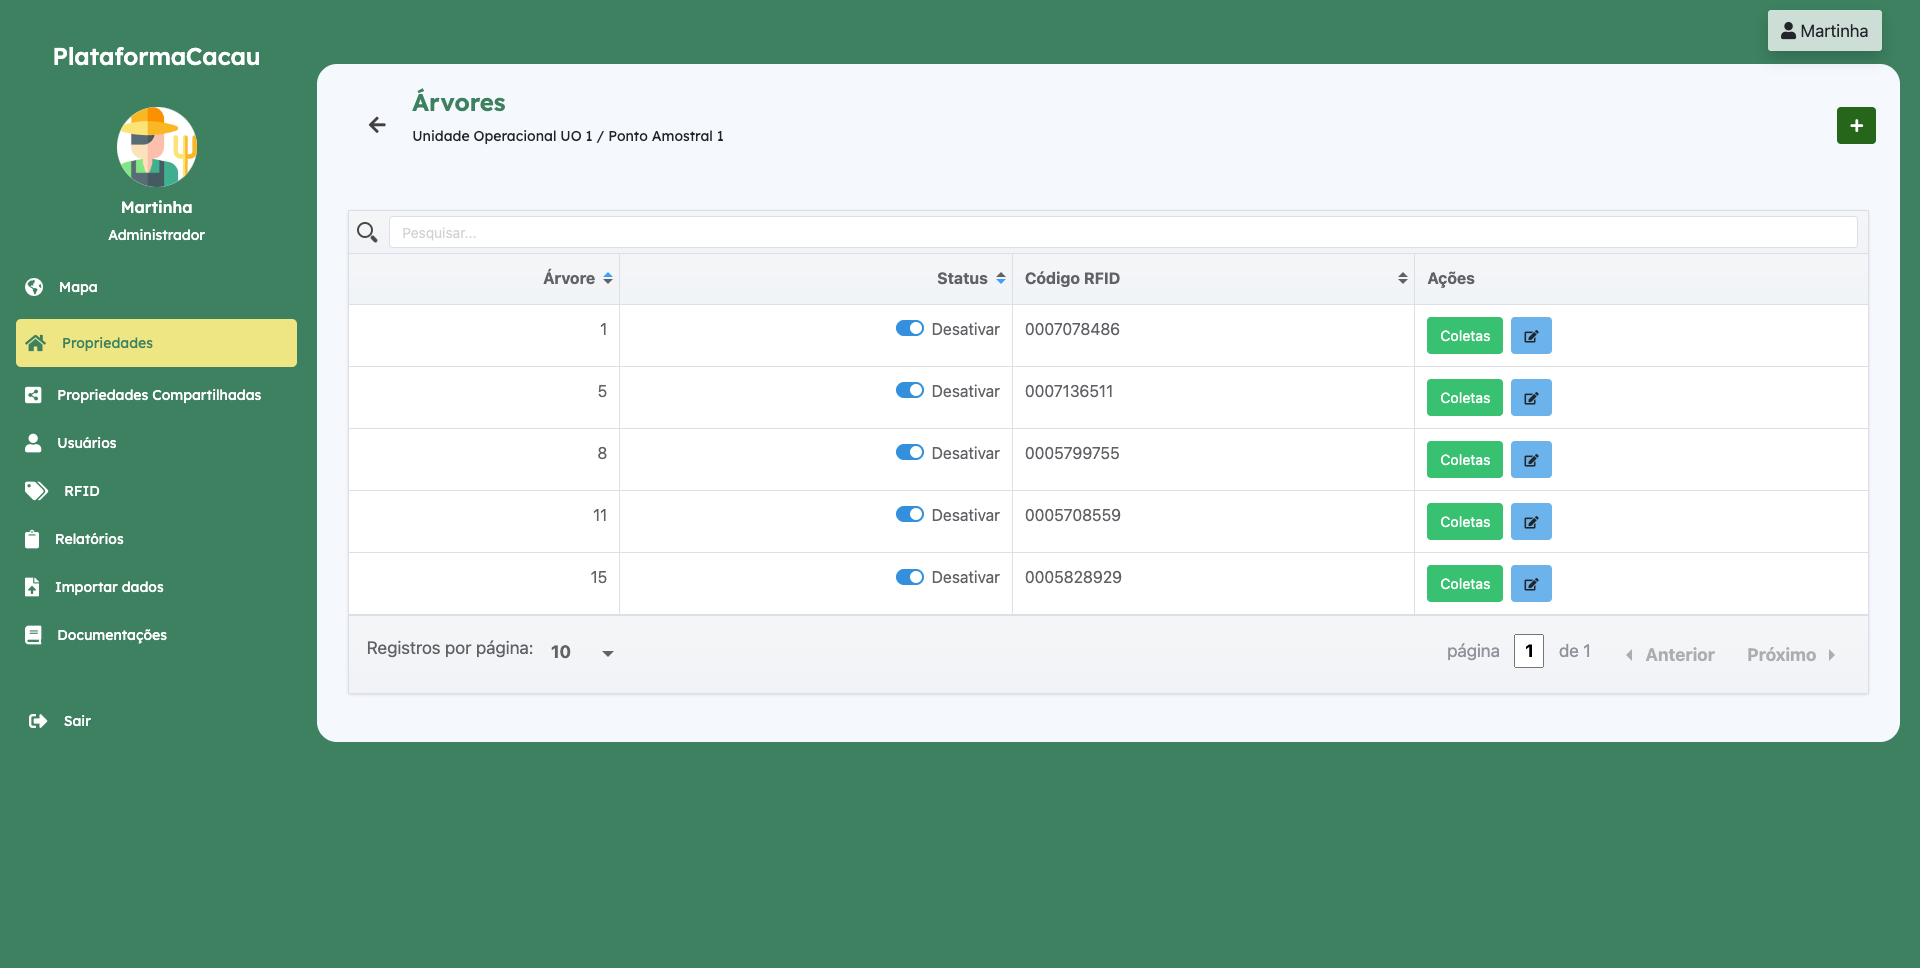
\includegraphics[width=\textwidth]{images/web/list-tree.png}}
 \caption{Janela de atualização do código RFID da árvore na plataforma web.}
 \label{fig:UpdateTreeRfid}
\end{figure}

\subsection{Imagens do Aplicativo Móvel}

\subsubsection{Telas de Listagem}
A Figura \ref{fig:ListScreens} inclui as telas de listagem de propriedades, unidades operacionais, áreas homogêneas, pontos amostrais e árvores, oferecendo uma navegação intuitiva para o coletor.

\begin{figure}[H]
    \centering
    \begin{minipage}[b]{0.30\textwidth}
        \centering
        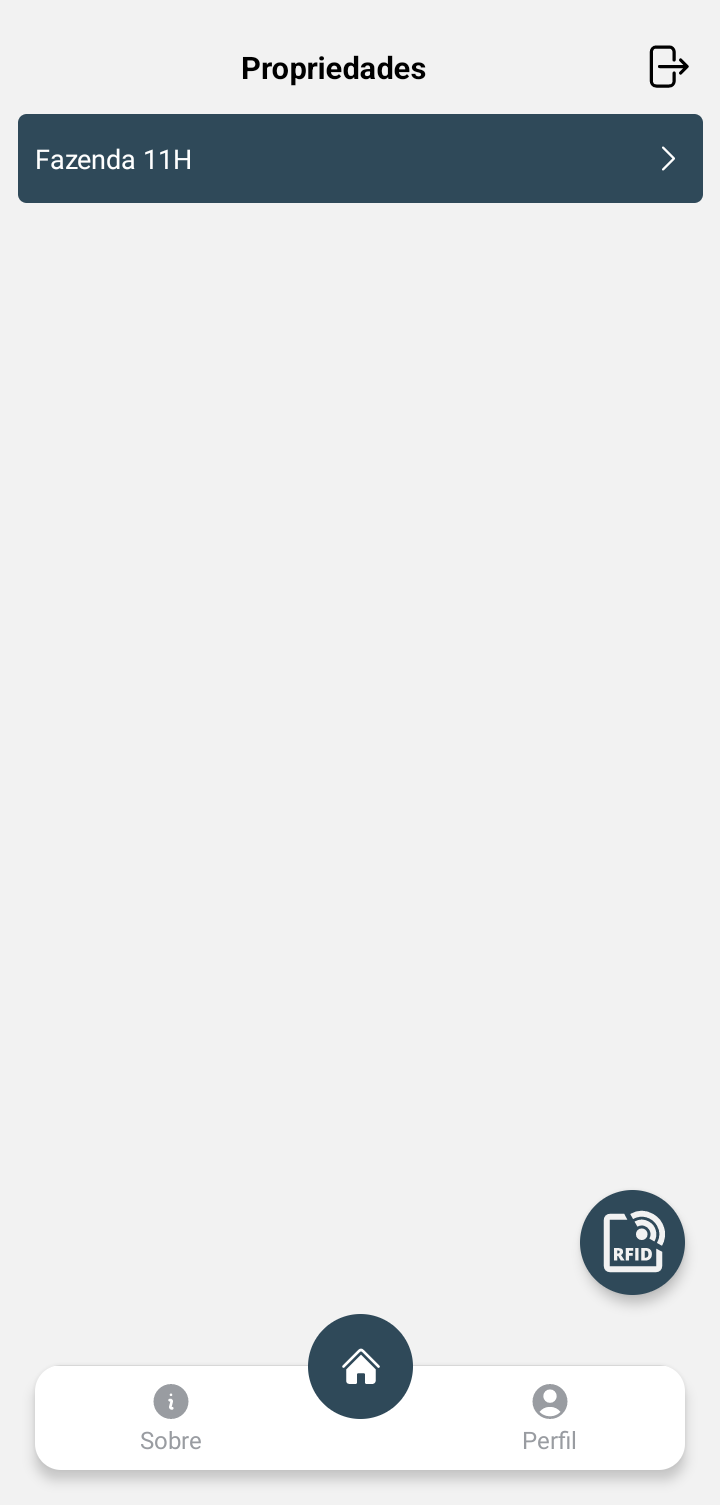
\includegraphics[width=\textwidth]{images/app/03-properties.png}
    \end{minipage}
    \hspace{3pt}
    \begin{minipage}[b]{0.30\textwidth}
        \centering
        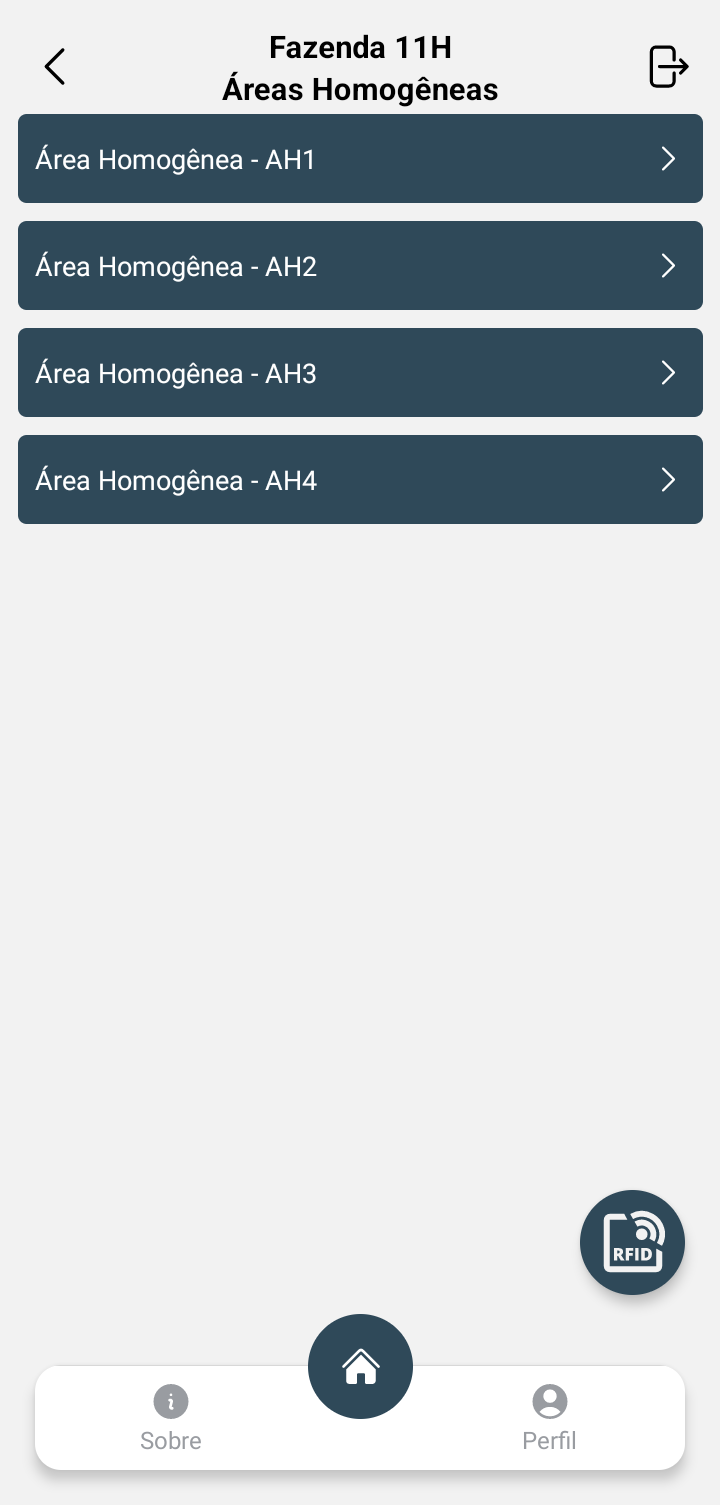
\includegraphics[width=\textwidth]{images/app/04-homogeneous-areas.png}
    \end{minipage}
    \hspace{3pt}
    \begin{minipage}[b]{0.30\textwidth}
        \centering
        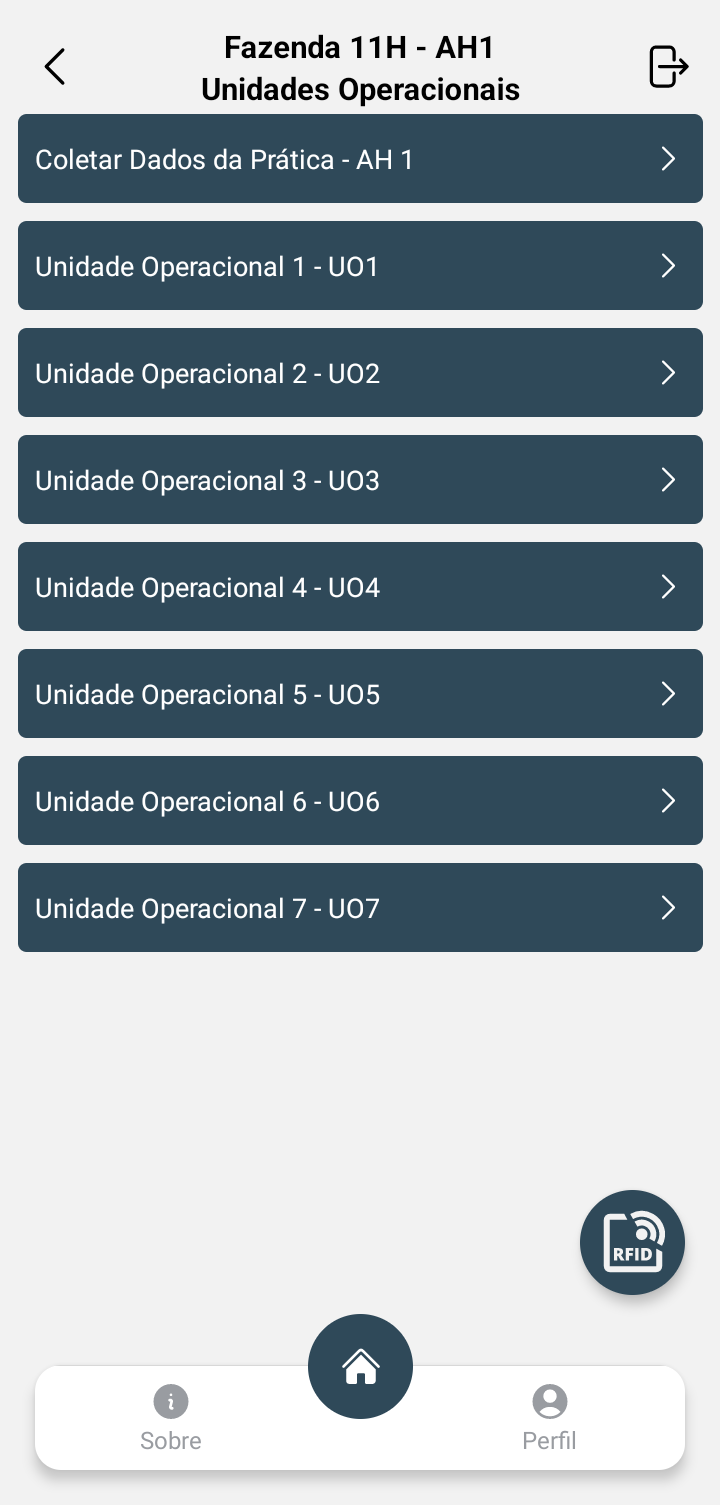
\includegraphics[width=\textwidth]{images/app/05-operational-units.png}
    \end{minipage}
    \hspace{3pt}
    \begin{minipage}[b]{0.30\textwidth}
        \centering
        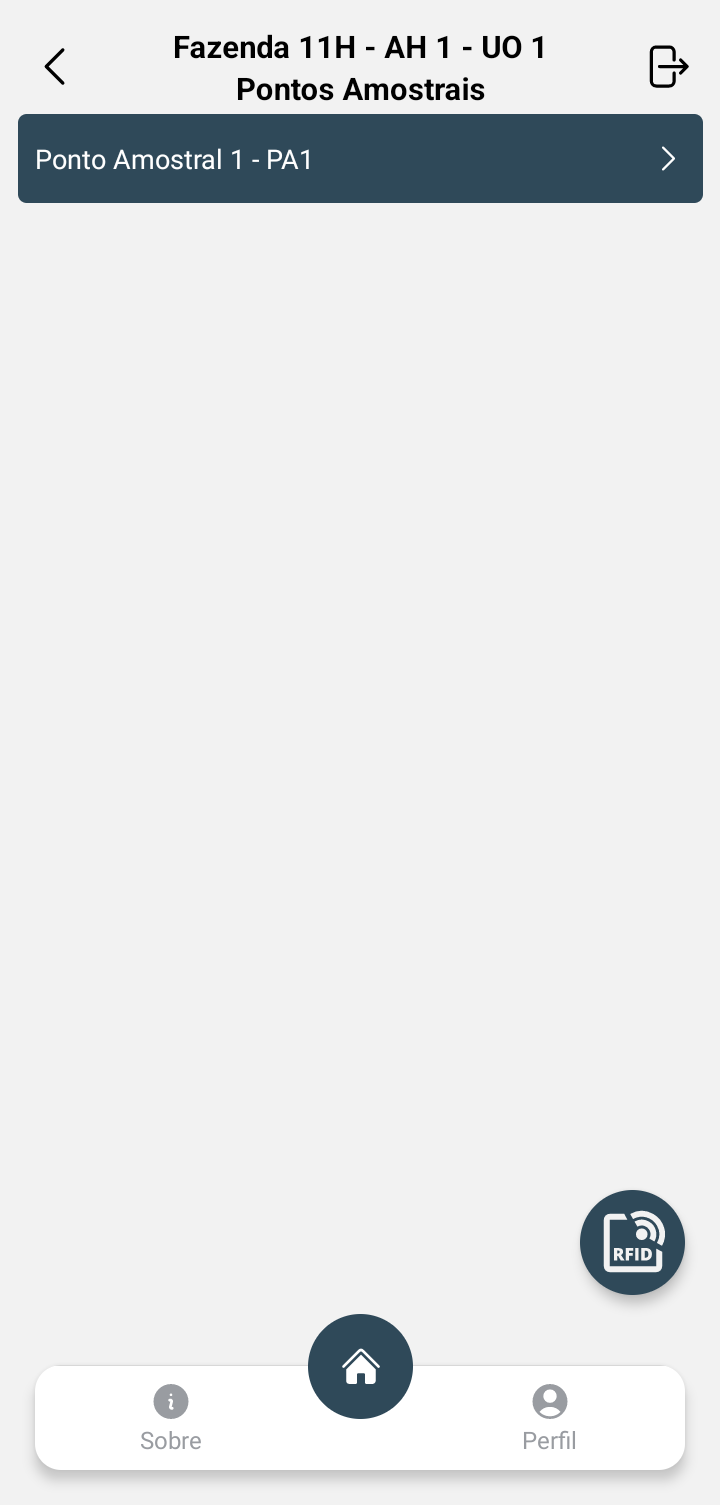
\includegraphics[width=\textwidth]{images/app/08-sampling-points.png}
    \end{minipage}
    \hspace{3pt}
    \begin{minipage}[b]{0.30\textwidth}
        \centering
        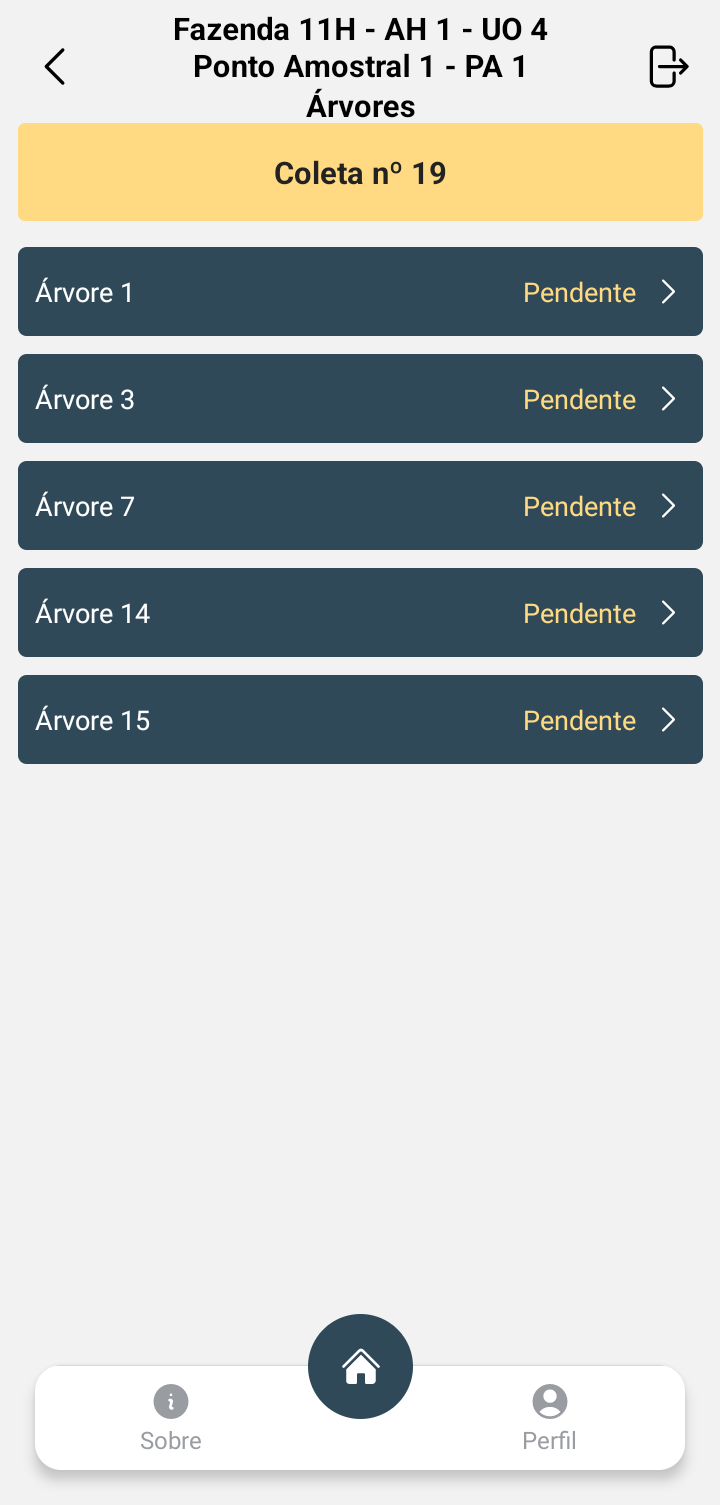
\includegraphics[width=\textwidth]{images/app/09-trees.png}
    \end{minipage}
    
    \caption{Telas de listagem do aplicativo móvel.}
    \label{fig:ListScreens}
\end{figure}

\subsubsection{Tela de Coleta dos Dados da Prática}
A Figura \ref{fig:PracticeDataScreen} representa a interface onde o coletor registra os dados gerais da área, incluindo condições de solo, presença de pragas, e outras informações relevantes sobre a saúde das plantas.

\begin{figure}[H]
    \centering
    \begin{minipage}[b]{0.30\textwidth}
        \centering
        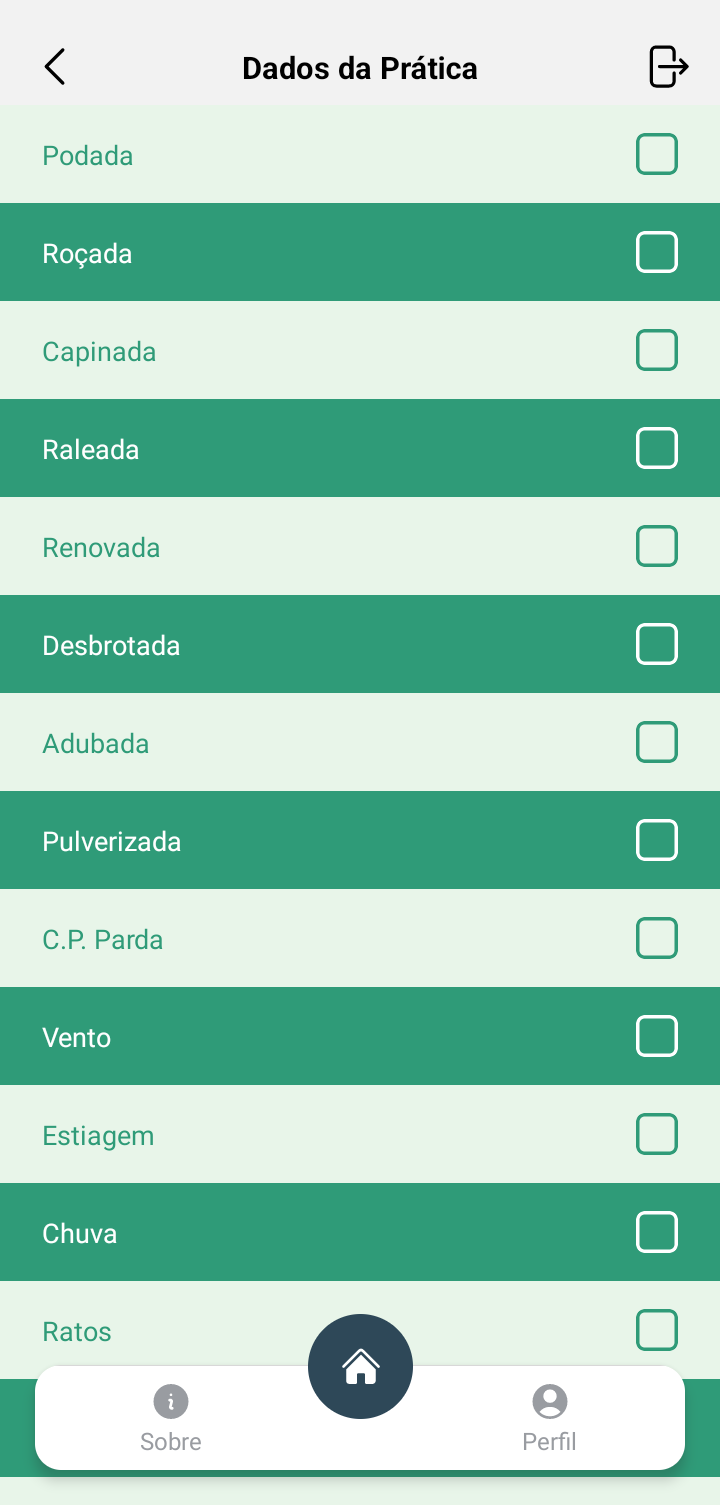
\includegraphics[width=\textwidth]{images/app/06-practice-data.png}
    \end{minipage}
    \hspace{5pt}
    \begin{minipage}[b]{0.30\textwidth}
        \centering
        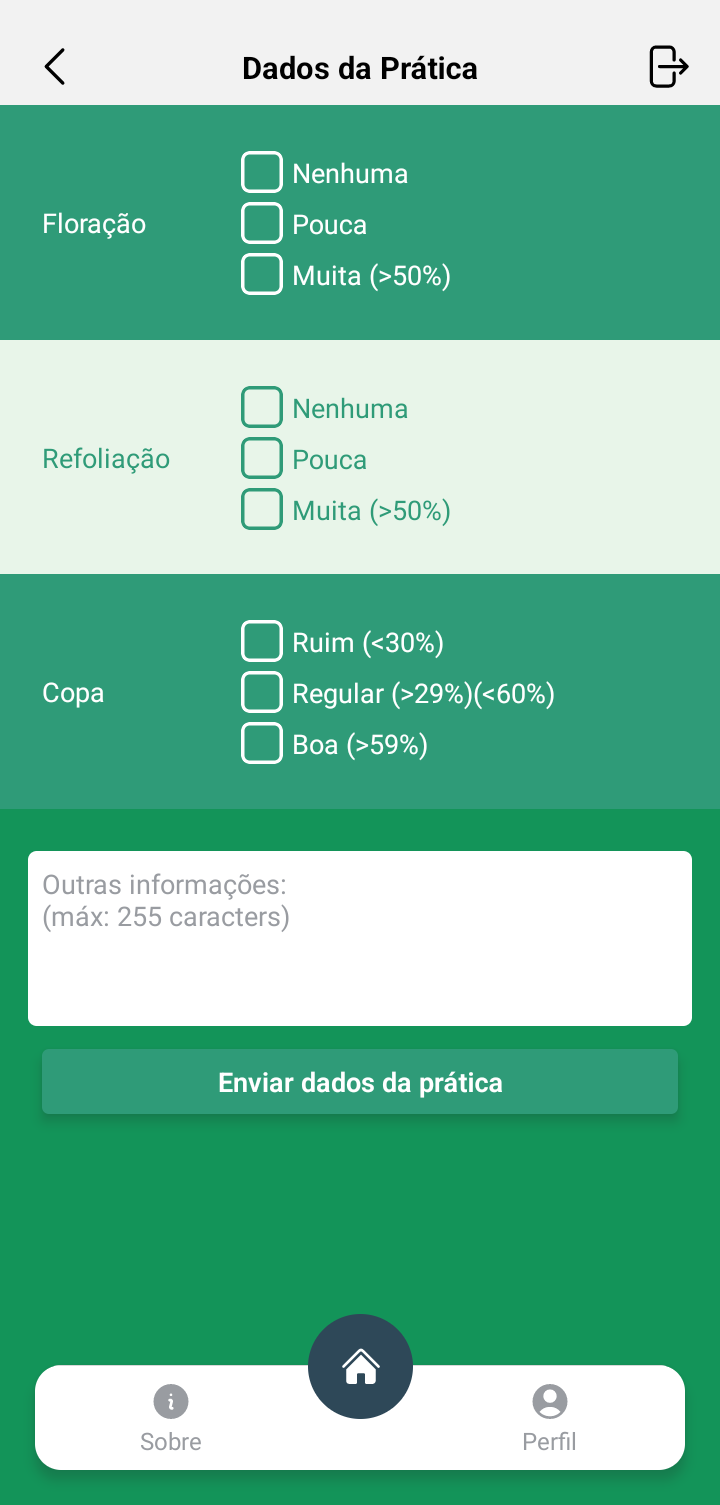
\includegraphics[width=\textwidth]{images/app/07-practice-data.png}
    \end{minipage}
    \hspace{5pt}
    
    \caption{Telas de coleta dos dados da prática no aplicativo móvel.}
    \label{fig:PracticeDataScreen}
\end{figure}

\subsubsection{Tela de Coleta dos Dados da Árvore}
A Figura \ref{fig:CollectDataScreen} representa a tela que permite ao coletor inserir dados específicos da árvore, como número de frutos e estágio de desenvolvimento, diretamente vinculado ao RFID da árvore.

\begin{figure}[H]
    \centering
    \begin{minipage}[b]{0.30\textwidth}
        \centering
        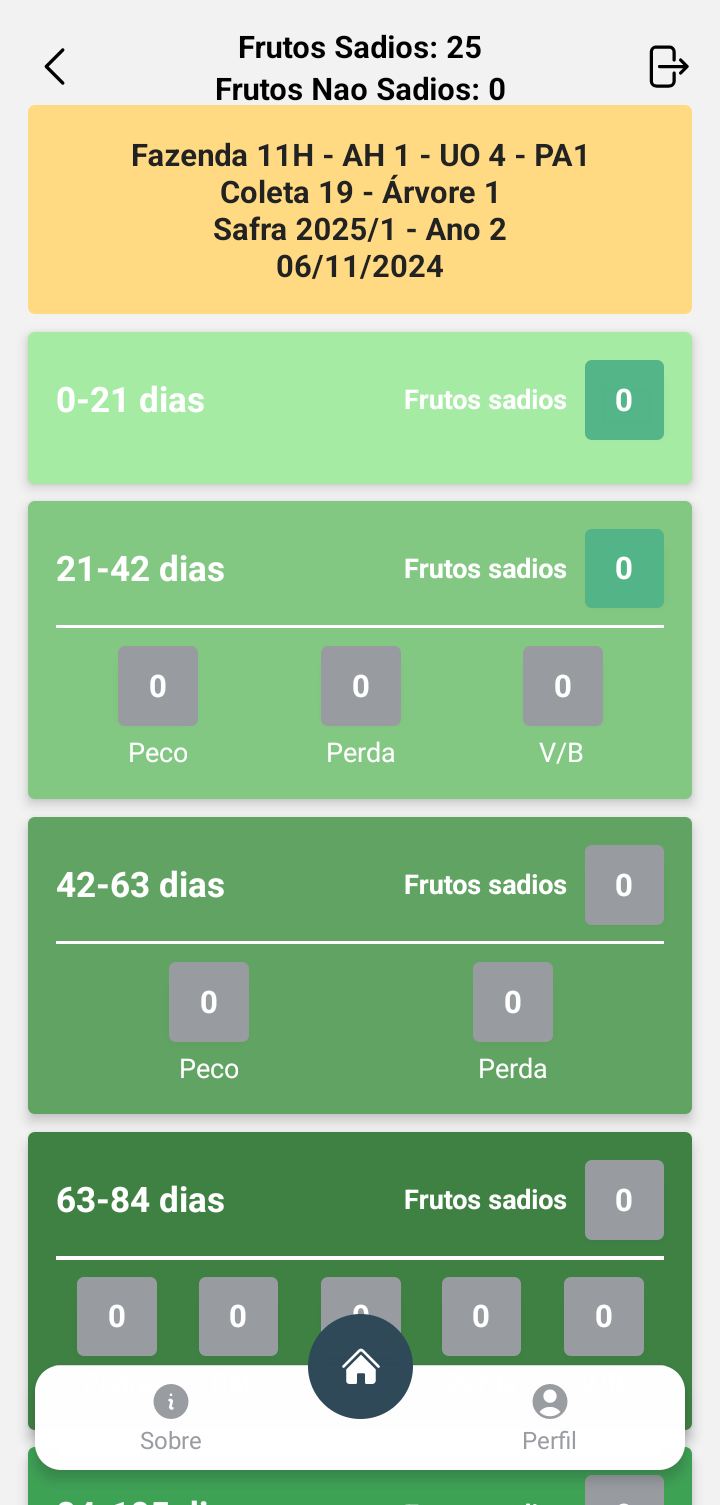
\includegraphics[width=\textwidth]{images/app/10-collect.png}
    \end{minipage}
    \hspace{3pt}
    \begin{minipage}[b]{0.30\textwidth}
        \centering
        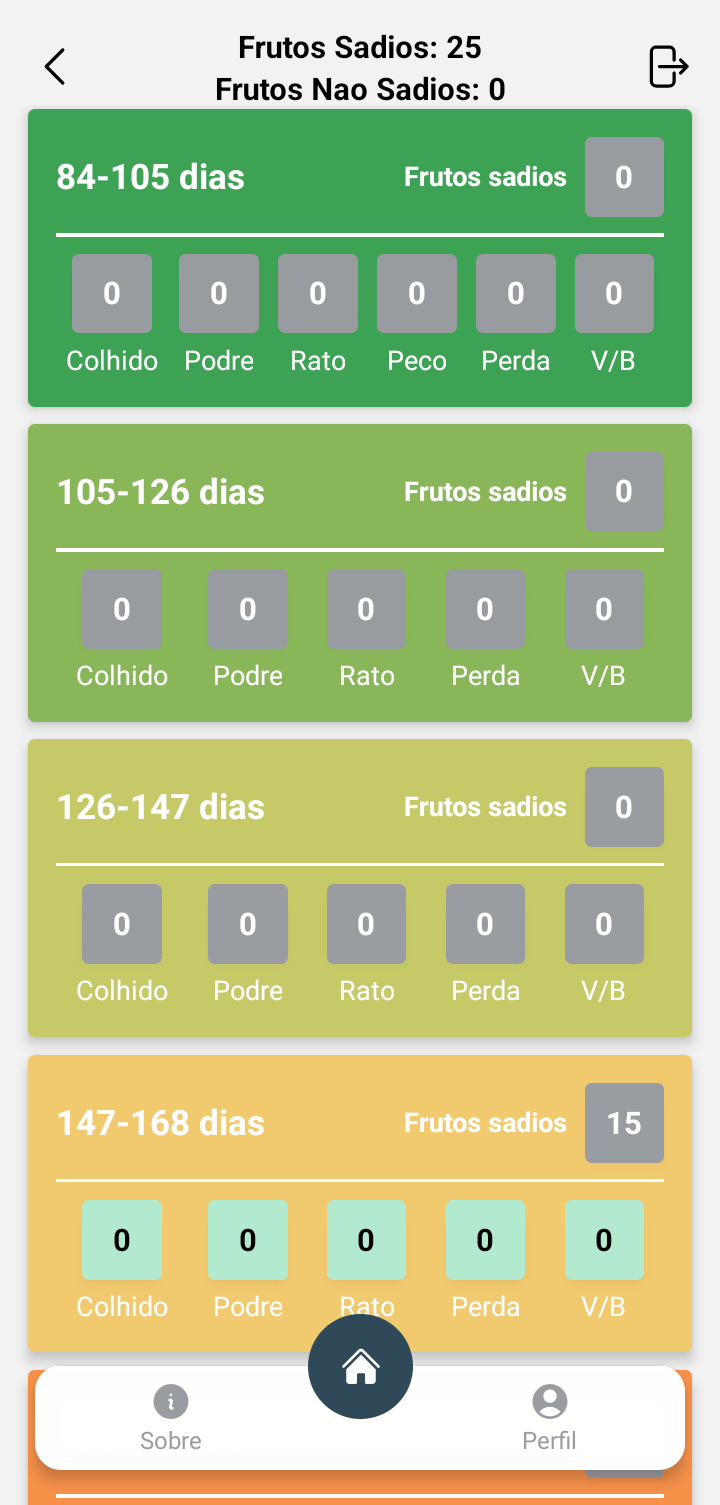
\includegraphics[width=\textwidth]{images/app/11-collect.png}
    \end{minipage}
    \hspace{3pt}
    \begin{minipage}[b]{0.30\textwidth}
        \centering
        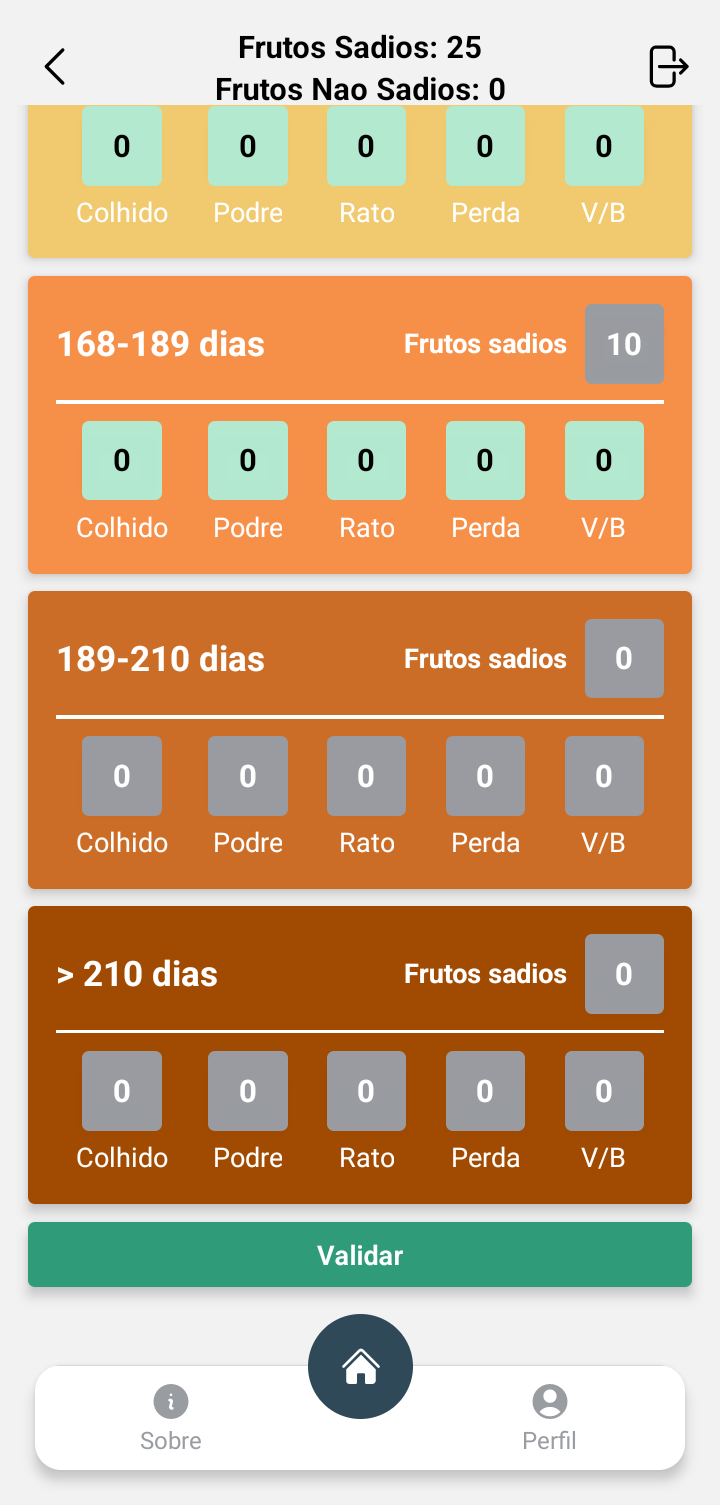
\includegraphics[width=\textwidth]{images/app/12-collect.png}
    \end{minipage}
    \hspace{3pt}
    
    \caption{Tela de coleta dos dados da árvore no aplicativo móvel.}
    \label{fig:CollectDataScreen}
\end{figure}


\subsection{Modal de Busca do RFID}
A Figura \ref{fig:RfidModal} representa o componente modal de busca de tags RFID que facilita a identificação das árvores durante a coleta, informando o RFID que está sendo pesquisado, agilizando o processo e minimizando erros de identificação. 

\begin{figure}[htb]
    \centering
    \begin{minipage}[b]{0.30\textwidth}
        \centering
        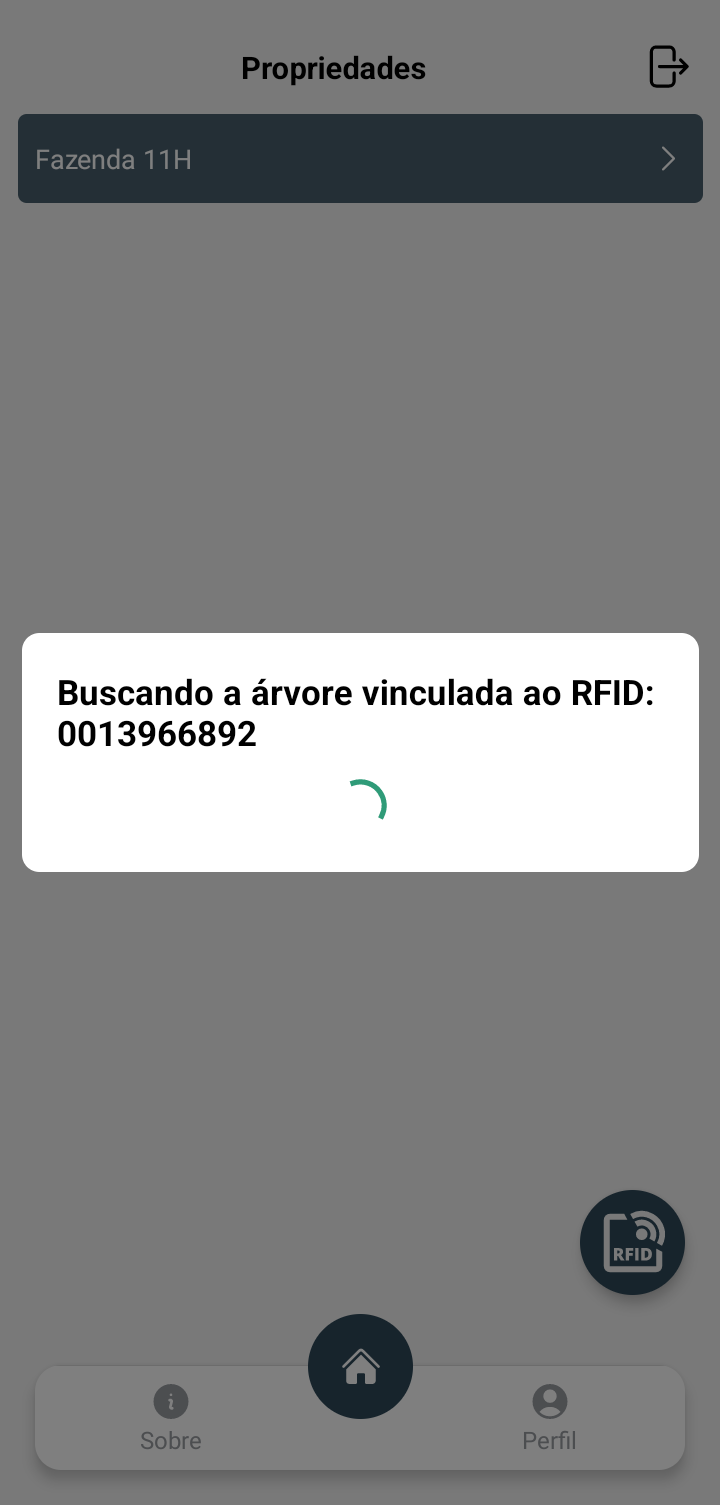
\includegraphics[width=\textwidth]{images/app/rfid-modal.png}
    \end{minipage}
    \caption{Modal de busca do RFID no aplicativo móvel.}
    \label{fig:RfidModal}
\end{figure}

Caso o ponto amostral já tenha sido visitado o aplicativo identifica este cenário e retorna uma mensagem informativa ao coletor. Este cenário pode ser visualizado na Figura \ref{fig:RfidSamplingPointVisitedMessage}

\begin{figure}[H]
    \centering
    \begin{minipage}[b]{0.30\textwidth}
        \centering
        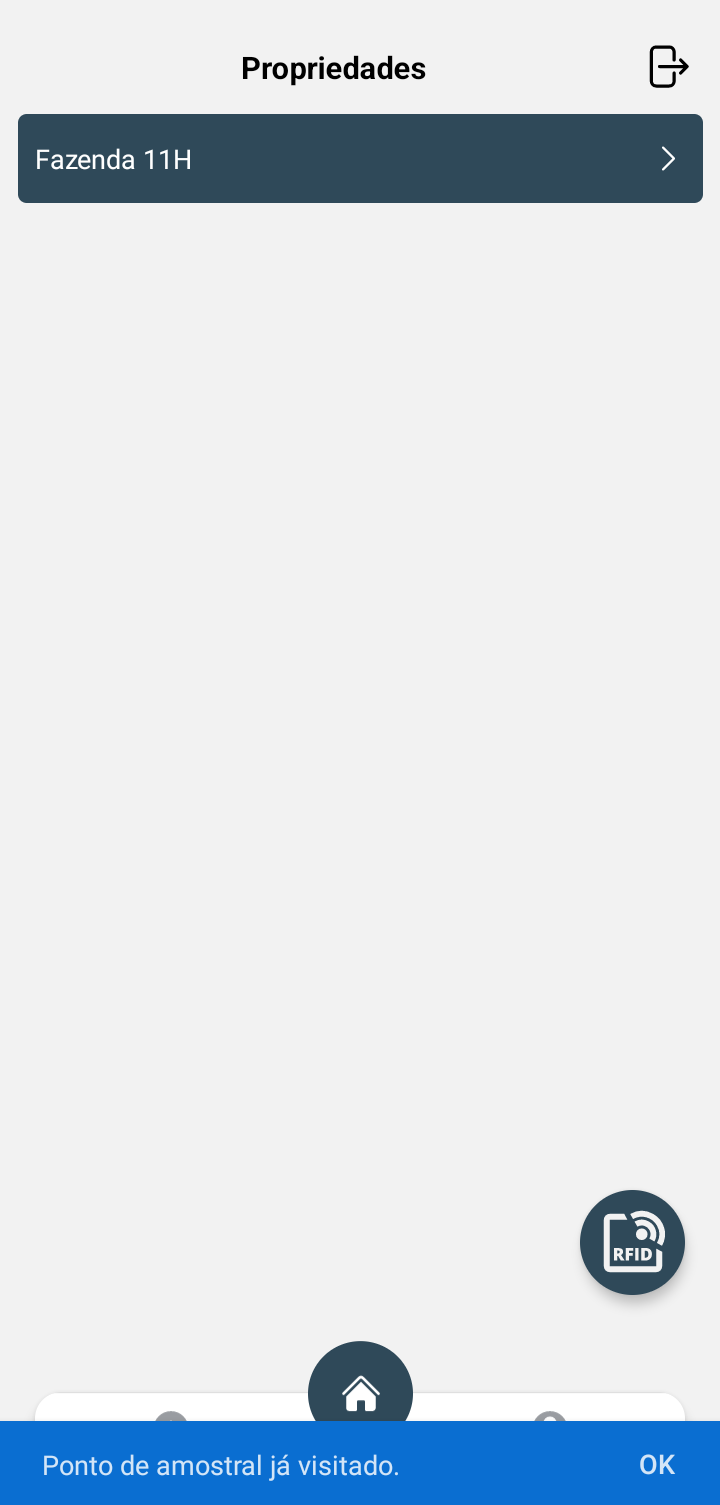
\includegraphics[width=\textwidth]{images/app/check-rfid-sp-visited.png}
    \end{minipage}
    \caption{Mensagem de busca do RFID indicando ponto amostral já visitado.}
    \label{fig:RfidSamplingPointVisitedMessage}
\end{figure}

\section{Estrutura de Dados e Funcionalidades da API}
Para garantir uma integração eficiente entre os diferentes módulos do ColetaCacau, foram implementadas funcionalidades adicionais na API e no banco de dados, descritas a seguir:

\subsection{Tabela de RFIDs Relacionada à Entidade de Árvores}
A tabela que armazena as tags RFID foi projetada para garantir a integridade dos dados e facilitar sua utilização no sistema, organizando as informações de forma clara e eficiente. Cada tag RFID está vinculada a uma árvore e pode também estar associada a um usuário responsável. Essa estrutura promove a rastreabilidade e consistência, essenciais para o funcionamento correto do ColetaCacau.

A principal característica dessa tabela é a unicidade dos códigos RFID. Cada código é único dentro do contexto da fazenda, isto é, só poderá existir um código RFID por fazenda mas, outras fazendas podem ter o mesmo código RFID. Além disso, as tags podem ser atualizadas ou desassociadas sem comprometer a integridade dos dados relacionados. Por exemplo, se uma fazenda ou usuário for excluído, a tag associada a ele não será removida, mas sim desvinculada, garantindo que os dados históricos sejam preservados.

A Figura \ref{fig:RfidTable} ilustra a organização e os relacionamentos dessa tabela no banco de dados, destacando como os registros de RFID interagem com outras entidades do sistema.

\begin{figure}[H]
    \centering
    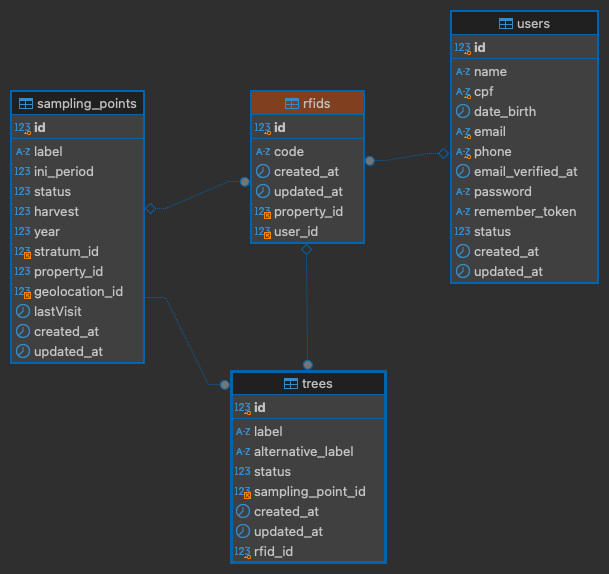
\includegraphics[width=0.8\textwidth]{images/database/rfid-table.png}
    \caption{Estrutura da tabela de RFIDs e seus relacionamentos no banco de dados.} \label{fig:RfidTable}
\end{figure}

\subsection{\textit{Endpoints} de Manipulação de RFIDs}
A API foi equipada com \textit{endpoints} específicos para realizar as operações de criação, atualização, listagem, visualização por ID, desassociação, exclusão e associação de RFIDs a uma árvore. Esses \textit{endpoints} oferecem flexibilidade e segurança no gerenciamento das tags, permitindo que o sistema se mantenha atualizado conforme as operações de campo evoluem.

\subsection{Exportação de Dados com RFID}
Foi incluído o campo de RFID relacionado a cada árvore na exportação de dados da coleta. Isso permite que os gestores tenham acesso a um relatório completo, incluindo a identificação única de cada árvore monitorada, o que facilita a análise de dados e o acompanhamento do progresso da safra ao longo do tempo.

\section{Discussão dos Testes e Resultados}
Os testes realizados demonstraram que o sistema ColetaCacau cumpre os requisitos de coleta de dados precisos e consistentes em campo, especialmente com a implementação de RFID e coleta \textit{offline}. As imagens apresentadas, tanto da plataforma web quanto do aplicativo móvel, reforçam a usabilidade e funcionalidade do sistema, demonstrando como cada funcionalidade contribui para a eficiência do trabalho dos coletores.

A redução significativa de tempo e a minimização de erros de identificação das árvores evidenciam os avanços obtidos com o uso de RFID, trazendo maior confiabilidade e eficiência à coleta de dados no campo. O sistema se mostra uma solução robusta para o monitoramento da safra de cacau, com potencial para ser expandido a outros contextos agrícolas no futuro.
